% Gerado por scripts/gerar_tabelas.py --- não editar à mão.
\begin{figure}[htbp]
    \centering
    \caption{Hiato salarial bruto por raça/cor e por sexo, 2007--2025}
    \label{fig:hiato-serie}
    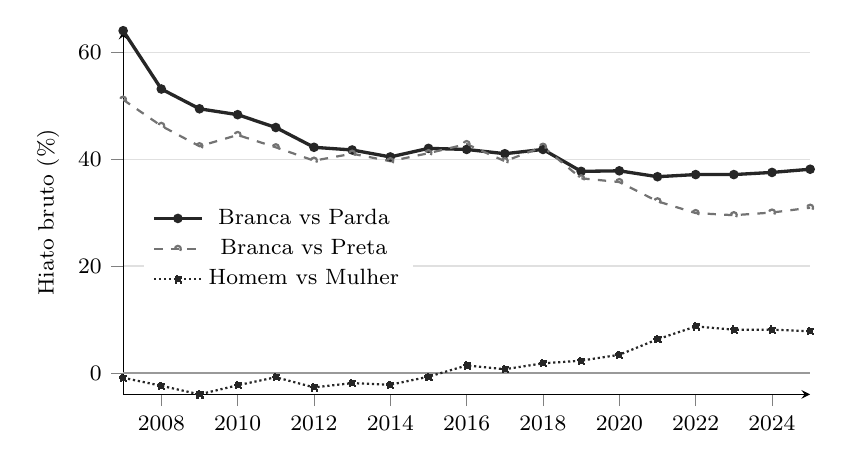
\begin{tikzpicture}
    \begin{axis}[width=\linewidth, height=6.2cm, axis lines=left, tick align=outside,
            ymajorgrids, grid style={black!12}, tick label style={font=\footnotesize},
            label style={font=\footnotesize}, title style={font=\small\bfseries},
            /pgf/number format/use comma, /pgf/number format/1000 sep={.}, width=0.85\textwidth, height=6.2cm, ylabel={Hiato bruto (\%)},
            xmin=2007, xmax=2025, xtick distance=2,
            x tick label style={/pgf/number format/1000 sep={}},
            legend style={font=\footnotesize, at={(0.03,0.40)}, anchor=west, draw=none, fill=white}]
        \addplot[black!40, thin, forget plot] coordinates {(2007,0) (2025,0)};
        \addplot[very thick, black!85, mark=*, mark size=1.1pt] coordinates {(2007,64.0) (2008,53.1) (2009,49.4) (2010,48.3) (2011,45.9) (2012,42.2) (2013,41.7) (2014,40.4) (2015,42.0) (2016,41.8) (2017,41.0) (2018,41.8) (2019,37.7) (2020,37.8) (2021,36.7) (2022,37.1) (2023,37.1) (2024,37.5) (2025,38.1)};
        \addlegendentry{Branca vs Parda}
        \addplot[thick, black!55, dashed, mark=o, mark size=1.1pt] coordinates {(2007,51.1) (2008,46.2) (2009,42.4) (2010,44.5) (2011,42.2) (2012,39.7) (2013,41.0) (2014,39.6) (2015,41.1) (2016,42.8) (2017,39.6) (2018,42.3) (2019,36.4) (2020,35.7) (2021,32.1) (2022,29.9) (2023,29.5) (2024,30.0) (2025,30.9)};
        \addlegendentry{Branca vs Preta}
        \addplot[thick, black!85, densely dotted, mark=square*, mark size=1.1pt] coordinates {(2007,-0.9) (2008,-2.4) (2009,-4.0) (2010,-2.3) (2011,-0.8) (2012,-2.7) (2013,-1.9) (2014,-2.2) (2015,-0.7) (2016,1.4) (2017,0.7) (2018,1.8) (2019,2.3) (2020,3.4) (2021,6.3) (2022,8.7) (2023,8.1) (2024,8.1) (2025,7.8)};
        \addlegendentry{Homem vs Mulher}
    \end{axis}
    \end{tikzpicture}
    \\[4pt]
    {\footnotesize Diferença percentual da remuneração média do primeiro grupo sobre a do segundo; negativo: o segundo grupo ganha mais. }Fonte: Autoria própria, a partir da camada Gold.
\end{figure}
